\documentclass[letterpaper,12pt]{article}
\usepackage{array}
\usepackage{geometry}
\geometry{letterpaper,tmargin=1in,bmargin=1in,lmargin=1.25in,rmargin=1.25in}
%\renewcommand\headrulewidth{0pt}
%\renewcommand\footrulewidth{0pt}
\usepackage{amsmath}
\usepackage{amssymb}
\usepackage{amsthm}
\usepackage{enumerate}
%\usepackage{harvard}
%\usepackage{setspace}
\usepackage{float,color}
\usepackage[pdftex]{graphicx}
\usepackage{hyperref}
\hypersetup{colorlinks,linkcolor=red,urlcolor=blue}
\theoremstyle{definition}
\newtheorem{theorem}{Theorem}
\newtheorem{acknowledgement}[theorem]{Acknowledgement}
\newtheorem{algorithm}[theorem]{Algorithm}
\newtheorem{axiom}[theorem]{Axiom}
\newtheorem{case}[theorem]{Case}
\newtheorem{claim}[theorem]{Claim}
\newtheorem{conclusion}[theorem]{Conclusion}
\newtheorem{condition}[theorem]{Condition}
\newtheorem{conjecture}[theorem]{Conjecture}
\newtheorem{corollary}[theorem]{Corollary}
\newtheorem{criterion}[theorem]{Criterion}
\newtheorem{definition}[theorem]{Definition}
\newtheorem{derivation}{Derivation} % Number derivations on their own
\newtheorem{example}[theorem]{Example}
\newtheorem{exercise}[theorem]{Exercise}
\newtheorem{lemma}[theorem]{Lemma}
\newtheorem{notation}[theorem]{Notation}
\newtheorem{problem}[theorem]{Problem}
\newtheorem{proposition}{Proposition} % Number propositions on their own
\newtheorem{remark}[theorem]{Remark}
\newtheorem{solution}[theorem]{Solution}
\newtheorem{summary}[theorem]{Summary}
%\numberwithin{equation}{section}
\bibliographystyle{aer}
\newcommand\ve{\varepsilon}
\newcommand\boldline{\arrayrulewidth{1pt}\hline}


\begin{document}

\begin{flushleft}
   \textbf{\large{Problem Set \#6}} \\
   MACS 40000, Dr. Evans \\
   Alexandre Sollaci
\end{flushleft}

\vspace{5mm}

\section*{Questions 1, 2, 3 and 4}

See appendix, figures 1-12 (in order).

Figure 12, the population growth rates in the economy, has a one time huge drop in growth. It looks weird, but the population dynamics in figure 11 seems correct. I do not know the source if this one time drop.

\section*{Question 5}

The values that characterize the Steady state are

\begin{verbatim}
{'C_ss': 7.1439448401484844,
 'EulErr_ss': array([ -7.76143594e-11,   8.99060826e-11,  -1.36965994e-11, ...,
          5.67101921e-11,  -2.55193200e-10,   5.89396976e-10]),
 'K_ss': array([ 17.79850383]),
 'RCerr_ss': array([ 0.45785928]),
 'Y_ss': array([ 9.02149359]),
 'b_ss': array([ 0.05425846,  0.1088026 ,  0.16366529, ...,  0.30400355,
         0.17075284,  0.06940022]),
 'c_ss': array([ 0.88125416,  0.8862201 ,  0.89117986, ...,  0.35421473,
         0.30842664,  0.26567508]),
 'r_ss': array([ 0.12740383]),
 'ss_time': 0.037582915565053554,
 'w_ss': array([ 0.93716503])}
\end{verbatim}

The Resource constraint error is way too big, probably due to a typo that I could not find. Notwithstanding, the solution seems to be correct. For the graph with the distribution of consumption and savings, see figure 13 in the appendix.


\clearpage
\appendix

\section{Figures}

\begin{figure}[h!]
\centering
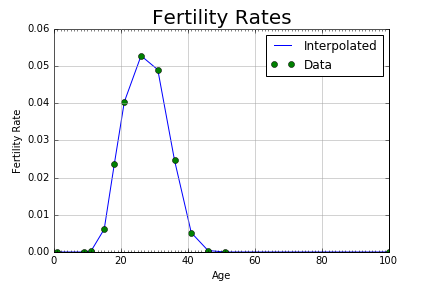
\includegraphics[scale=.8]{code/images/fert_rate}
\caption{Distribution of fertility rates by age, 100 years lived agent.}
\end{figure}

\begin{figure}[h!]
\centering
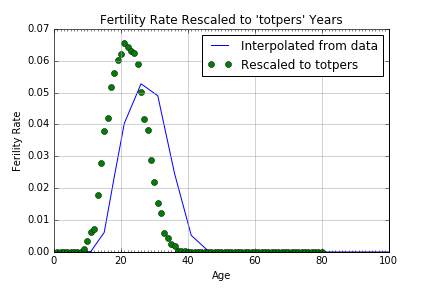
\includegraphics[scale=.8]{code/images/fert_totpers80}
\caption{Distribution of fertility rates by age: comparison between 100 and 80 periods of life.}
\end{figure}

\begin{figure}[h!]
\centering
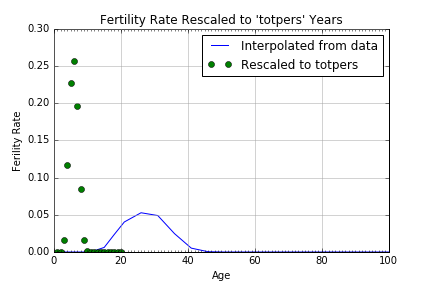
\includegraphics[scale=.8]{code/images/fert_totpers20}
\caption{Distribution of fertility rates by age: comparison between 100 and 20 periods of life.}
\end{figure}


\begin{figure}[h!]
\centering
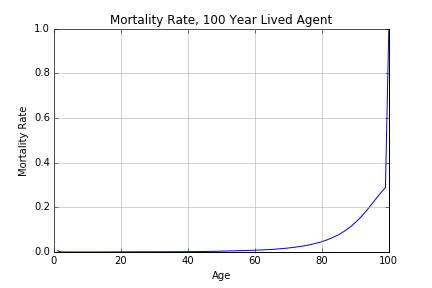
\includegraphics[scale=.8]{code/images/mort_totpers100}
\caption{Distribution of mortality rates by age, 100 years lived agent.}
\end{figure}

\begin{figure}[h!]
\centering
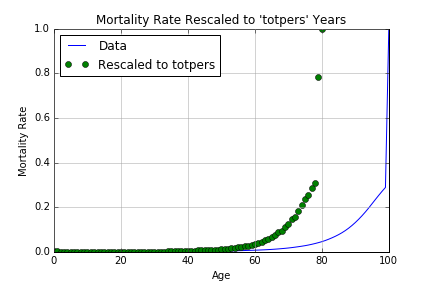
\includegraphics[scale=.8]{code/images/mort_totpers80}
\caption{Distribution of mortality rates by age: comparison between 100 and 80 periods of life.}
\end{figure}

\begin{figure}[h!]
\centering
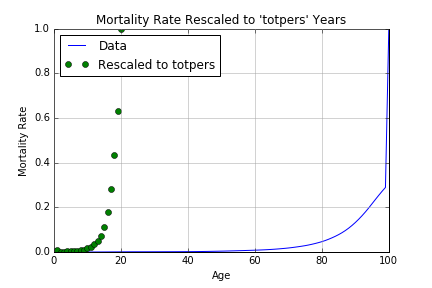
\includegraphics[scale=.8]{code/images/mort_totpers20}
\caption{Distribution of mortality rates by age: comparison between 100 and 20 periods of life.}
\end{figure}


\begin{figure}[h!]
\centering
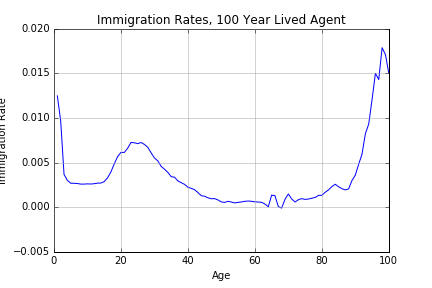
\includegraphics[scale=.8]{code/images/imm_totpers100}
\caption{Distribution of immigration rates by age, 100 year lived agent.}
\end{figure}

\begin{figure}[h!]
\centering
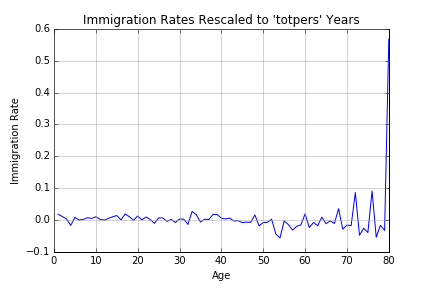
\includegraphics[scale=.8]{code/images/imm_totpers80}
\caption{Distribution of immigration rates by age, 80 period lived agent.}
\end{figure}

\begin{figure}[h!]
\centering
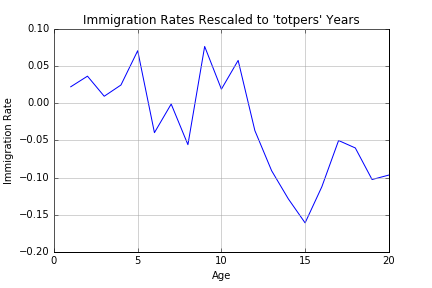
\includegraphics[scale=.8]{code/images/imm_totpers20}
\caption{Distribution of immigration rates by age, 20 period lived agent.}
\end{figure}

\begin{figure}[h!]
\centering
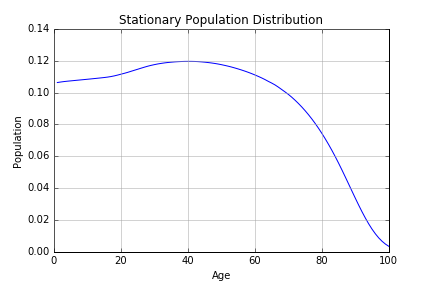
\includegraphics[scale=.8]{code/images/stat_pop}
\caption{Steady-state stationary population distribution, $\bar{\omega}_s$.}
\end{figure}

\begin{figure}[h!]
\centering
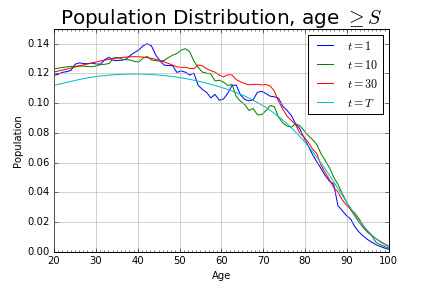
\includegraphics[scale=.8]{code/images/stat_pop_T}
\caption{Stationary population distribution at times $t = 1, 10, 30$, and $T=200$.}
\end{figure}

\begin{figure}[h!]
\centering
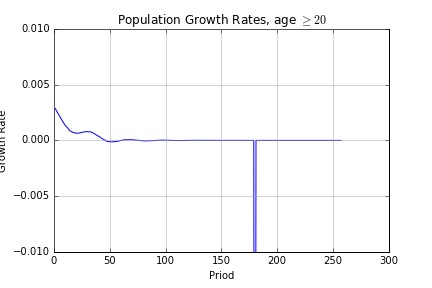
\includegraphics[scale=.8]{code/images/growth_rate_pop}
\caption{Population growth rate of the economically relevant population.}
\end{figure}

\begin{figure}[h!]
\centering
\includegraphics[scale=.8]{code/images/ss_bc}
\caption{Steady-state distribution of consumption and savings.}
\end{figure}

\end{document}



